\documentclass{article}

% if you need to pass options to natbib, use, e.g.:
%     \PassOptionsToPackage{numbers, compress}{natbib}
% before loading neurips_2019

% ready for submission
% \usepackage{neurips_2019}

% to compile a preprint version, e.g., for submission to arXiv, add add the
% [preprint] option:
%     \usepackage[preprint]{neurips_2019}

% to compile a camera-ready version, add the [final] option, e.g.:
     \usepackage[final]{neurips_2019}

% to avoid loading the natbib package, add option nonatbib:
%     \usepackage[nonatbib]{neurips_2019}

\usepackage[utf8]{inputenc} % allow utf-8 input
\usepackage[T1]{fontenc}    % use 8-bit T1 fonts
\usepackage{hyperref}       % hyperlinks
\usepackage{url}            % simple URL typesetting
\usepackage{booktabs}       % professional-quality tables
\usepackage{amsfonts}       % blackboard math symbols
\usepackage{nicefrac}       % compact symbols for 1/2, etc.
\usepackage{microtype}      % microtypography
\usepackage[square,sort,comma,numbers]{natbib}
\usepackage{appendix}
\usepackage{graphicx}
\usepackage{epstopdf}
\usepackage{inputenc}
\usepackage{subfig}
% \usepackage{float}
% \usepackage{geometry}
% \usepackage{float}
\renewcommand\refname{}
\title{CWAS: DeepSEA Prioritization of Cancer Mutations}

% The \author macro works with any number of authors. There are two commands
% used to separate the names and addresses of multiple authors: \And and \AND.
%
% Using \And between authors leaves it to LaTeX to determine where to break the
% lines. Using \AND forces a line break at that point. So, if LaTeX puts 3 of 4
% authors names on the first line, and the last on the second line, try using
% \AND instead of \And before the third author name.

\author{%
  George Henderson, Michael Khachatrian, Samson Petrosyan\\
  Department of Electrical Engineering and Computer Science\\
  University of California, Berkeley\\
  Berkeley, CA 94704 \\
  % examples of more authors
  % \And
  % Coauthor \\
  % Affiliation \\
  % Address \\
  % \texttt{email} \\
  % \AND
  % Coauthor \\
  % Affiliation \\
  % Address \\
  % \texttt{email} \\
  % \And
  % Coauthor \\
  % Affiliation \\
  % Address \\
  % \texttt{email} \\
  % \And
  % Coauthor \\
  % Affiliation \\
  % Address \\
  % \texttt{email} \\
}

\begin{document}

\maketitle

\begin{abstract}
  Our approach uses the Flatiron Institute's DeepSEA neural network to produce a novel method of cancer-associated mutation prioritization. Beginning with mutation sets from the Sanger Institute's Cancer Browser, this approach identifies mutated cell lines with high significance thresholds across DeepSEA's feature predictions. In the process of this, we propose methods to automate the interface with DeepSEA in order to support predictions on sequence sets that otherwise would be too large to input to DeepSEA manually. We propose alternate prioritizations for sequence segments in pancreatic, lung, breast, and bone cancer types.
\end{abstract}


\section{Introduction}
It was discovered that the majority of diseases are caused by noncoding genomic variations at a single-nucleotide resolution \cite{1}. Genome-wide association study (GWAS) has proven to be a reliable technique for identifying genetic risk factors by  identifying correlated genetic mutations and proposing potentially causative elements in diseases to which the method is applied \cite{2}. The identification of the \textit{Complement Factor H} as a major risk-factor for age-related macular degeneration was one of the earlier successes of GWAS \cite{3, 4, 5}. Notwithstanding  its early successes, scientists and researchers have raised a number of issues with GWAS \cite{2}. Specifically, a lack of biological relevance has been a predominant theme among these critiques \cite{6, 7, 8}. 

The application of convolutional neural networks (CNNs) to DNA sequence analysis has been shown to surpass more established algorithms at predicting epigenetic features, as they identify  potential functional significance from the chosen inputs \cite{9, 10}. Specifically, Zhou and Troyanskaya have developed a deep learning model - titled DeepSEA - that predicts the noncoding-variant effects \textit{de novo} from sequence by directly learning a regulatory sequence code from chromatin-profiling data with single nucleotide sensitivity \cite{10}. The ability of DeepSEA to predict chromatin effects of sequence alteration with single-nucleotide sensitivity was the driving reason we set out to develop a new framework, one which incorporated both disease correlation and inferential modelling of biological function: a cancer-wide association study (CWAS). 

\section{Methods}

\subsection{Identifying Datasets}
Locating datasets which we could use in our analysis presented the project's first major hurdle. The initial experimental design was to take SNPs that had been identified as significant from GWAS, input them into DeepSEA, and thus to add to GWAS a summary understanding of functional noncoding elements at GWAS-significant loci.  

This design presented two immediate issues. First, when DeepSEA receives a VCF as input, it does not produce a readout of epigenetic feature predictions; it instead produces a risk score. Therefore, taking a filtered VCF of SNPs which we had identified from a lung cancer GWAS, for example, would cause DeepSEA to return a positive statement that, yes, these SNPs are implicated in lung cancer. Using DeepSEA in the manner in which the group had originally intended would propose to provide no new meaningful inferences, only circular confirmations as to cancer correlation. 

The second issue with the group's intended approach is that, when DeepSEA receives a VCF, it is specified to accept only noncoding variants. The input VCF would therefore have to be queried against a file indicating which genomic regions are coding and which are noncoding. Our group expected that, if we had constructed a reference system to filter GWAS-significant SNPs for their coding or non-coding identity, we would risk reducing the GWAS-significant SNPs to a proportion of the VCF which excluded the main body of the correlated variants.

The optimal input to DeepSEA was found to be the Fasta file format. With this, we would produce from DeepSEA the epigenetic feature predictions which we had originally sought. Our group felt that the Sanger Institute's Catalogue of Somatic Mutations in Cancer (COSMIC) recommended itself to our datatype constraints and to our research question. At COSMIC's data download site, we found a file including all Fasta-type sequence segments which COSMIC had collected. This included over 50,000 sequence segments from cancer subjects. Immediately identifying that this input size exceeded DeepSEA's processing limitations, it became necessary to consider not only an automated data processing system for interface with DeepSEA, but also a system of subsetting the main Fasta to conduct analyses on narrower sets of mutated sequences.

For this, we used the COSMIC Cancer Browser. Since our group was interested in comparing functional noncoding elements across different cancer types, we queried the Cancer Browser for cancer types by organ or region affected, its most inclusive category. Navigating to lung cancer, for example, the Cancer Browser provides summary statistics on the genes which have been sequenced and identified as mutated or unmutated for this cancer type. From here, we downloaded CSV's for cancer types of interest, which encoded the gene of interest, the number of mutated samples sequenced, and the number of total samples sequenced. In the next section, we discuss the process by which we applied this CSV to subset the Fasta we had downloaded from COSMIC.

\subsection{Mapping Mutations Types to Sequences}
The COSMIC Cancer Browser data presented a challenge since while it contains the names of the genes associated with cancers of various tissues, it does not contain the actual genetic sequences of these tissues. 
The actual sequences for the genes can be found in the Data Downloads page in the COSMIC Cancer Browser - however it is one large file that contains data on all the sequences for every sort of gene they have data on - rather than discriminating between cancer types. Therefore, it was necessary to compile the sequences for each cancer type.

To accomplish this, we wrote a script, \texttt{breakdown.py}, that goes through the cancer-specific files from the COSMIC cancer browser and queries the file containing the sequences for all of the genes. The sequences for the cancer-specific genes are then compiled into a file. 



\subsection{Breaking Down Files}
While DeepSEA provides a web-hosted graphical user interface (GUI) for uploading a variety of genomic files (i.e. \texttt{fasta}, \texttt{vcf}) it also puts a capacity on these file sizes. Thus, a single file upload that is larger than 1 MB, specifically 20,000 lines, will not yield any results. This serves as a significant obstacle as the majority of files identified are larger than 20,000 lines.

To overcome memory limitations, \texttt{breakdown.py} splits the cancer-specific sequence files into multiple smaller files that can be uploaded to DeepSEA.

After following the \href{https://github.com/sme777/seaWAS/blob/master/README.md}{instructions} on local environment set up, \texttt{breakdown.py} can be run in the following format: 
% hIn order to run \texttt{breakdown.py}, it must be put in a common directory with the file containing the cancer-specific genes and the file containing the sequences for all the genes (both in \texttt{.txt} format). Then, the command 
\begin{center}
\texttt{python3 breakdown.py \{filename of file containing sequences for all genes\} \{filename of file containing cancer specific genes\} \{number of desired sequences per output file\}}
\end{center}
will generate a directory \texttt{fasta\_files} which will contain the desired files.

\subsection{Integrating DeepSEA}
At its current state, DeepSEA supports GUI and scriptable API. While it’s more intuitive and easier to interact with DeepSEA’s GUI, the task becomes cumbersome when the number of files to upload exceeds 100 and can often take several hours to finish. Its counterpart API seems to provide an alternative and more scalable solution, however, it was discovered during this project that the API does not support POST requests - though stated otherwise in the documentation - which is necessary to upload and make any submission to the service. With no efficient solutions left, we decided to write our own script which would automate the process of making a submission to the DeepSEA microservice.

The script is written in python and utilizes the \texttt{selenium} webdriver library. In the most general form the script can be run by downloading the file and typing the following instructions in the \href{https://github.com/sme777/seaWAS/blob/master/README.md}{README file}. In the most general form, one would type the following command in the terminal:
\begin{center}
\texttt{python3 web.py -{}-windows 100 -{}-folder lung\_cancer/fasta -{}-path lung\_cancer/results -{}-cancer lung}
\end{center}
The line above will open a Firefox window and for each of 100 files upload the selected \texttt{fasta} files, wait for DeepSEA to finish processing, and download the generated compressed (\texttt{tar.gz}) file. The results will be saved into \texttt{lung\_cancer/results} folder. All of the flags starting with \texttt{-{}-} are optional, and it is possible to run a script by just typing \texttt{python3.py web.py} although the script will look for files in a default folder and download to a default folder.

It's possible to run the script on multiple terminals at once. For example, for five different cancer types one can open five different terminals and run the command with different input folders. It's important to specify the output folder in this case as otherwise results will be saved to the default folder and it will not be possible to differentiate between results for different cancer types because of DeepSEA's file naming conventions.

\subsection{Extracting and Merging Probability Tables}
The \texttt{web.py} script takes the longest amount of time to run (in minutes) as it depends on external service, however, filtering still needs to be done before the data is ready for analysis. Specifically, the first obstacle we faced was extracting the associated probability table for all features from the list of compressed files, and second merging these tables together for each cancer type. 

When done manually by hand this process can take up to an hour for the results generated by only 20 \texttt{fasta} files. The amount of time necessary to work with larger number of files can range from several hours to a day. Here, we provide another script which automates the process and shrinks the amount of time to milliseconds. Extensive documentation on how to run the script can be found in the \href{https://github.com/sme777/seaWAS/blob/master/README.md}{repository} of the project. In the most general form, one would type the following command in the terminal:
\begin{center}
\texttt{python3 concat.py lung\_cancer/results -{}-cancer lung}
\end{center}
The script will start by extracting the \texttt{tsv} probability tables from the compressed files located in the \texttt{lung\_cancer/results} directory, followed by merging these \texttt{tsv} files and removing any miscellaneous column headers. The output is a single \texttt{tsv} file consisting of probabilities of features for all cancer mutations.
\section{Discussion}
Once data collection and data processing were complete, we obtained tabular data which indicated the predicted feature probabilities for the input cell lines. We began with the intention to identify patterns across cancer types as far as epigenetic features. What, for example, would the epigenetic state of mutated lung cancer cell lines have in common with cell lines from breast cancer? 

All initial analyses were undertaken on data processing notebooks specific to the cancer type for which we had produced a complete feature prediction matrix. These feature prediction matrices represent the aggregate output from DeepSEA for a given cancer type. To identify patterns in the represented features, we began analysis by summing across all columns. This approach yielded informative results, but these results were not actionable for our study. 

\begin{figure}[h!] 
    \centering
    \subfloat[Breast Cancer Gene Sums]{%
        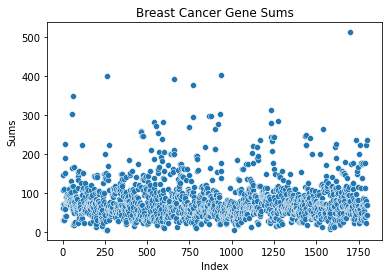
\includegraphics[width=0.40\textwidth]{figures/breast_cancer_feature_sum.png}%
        \label{fig:a}%
        }%
    \hfill%
    \subfloat[Breast Cancer Feature Sums]{%
        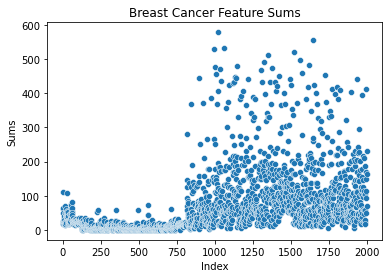
\includegraphics[width=0.40\textwidth]{figures/breast_cancer_gene_sum.png}%
        \label{fig:b}%
        }%
    \caption{Gene-specific and epigenetic feature-specific probability sums.}
\end{figure}
We see in the plot that a category boundary exists at which  probabilities display dramatic enrichment. This is where the set changes from probabilities of DNase features to probabilities of histone modifications. By taking the fifth percentile of total feature probability, we found that the DeepSEA outputs did not associate strongly with any particular cell type. This was to be expected, but the inconsistencies of cell types included in the top five percent of features indicated that the feature probability matrix would be better used to perform gene-wide, rather than feature-wide, thresholding. 

In Breast Cancer Feature Sums, once the category boundary is passed, the data appear similar to a Manhattan plot. In Breast Cancer Gene Sums, we have a plot that is more consistent with our expectations of the probability sum distribution. Seeing this plot, we identified that the row sums, or the sum of probabilities by input gene, would be informative as to cross-cancer patterns. Note that the concept of mutation prioritization, to a large extent, begins here. Having identified that the cell-type outputs for chromatin marks present insufficient cell-type consistency for use in our association study, we identify the sum of feature probabilities by gene as a marker of mutation effect size. 
\begin{figure}[h!]
  \makebox[\textwidth][c]{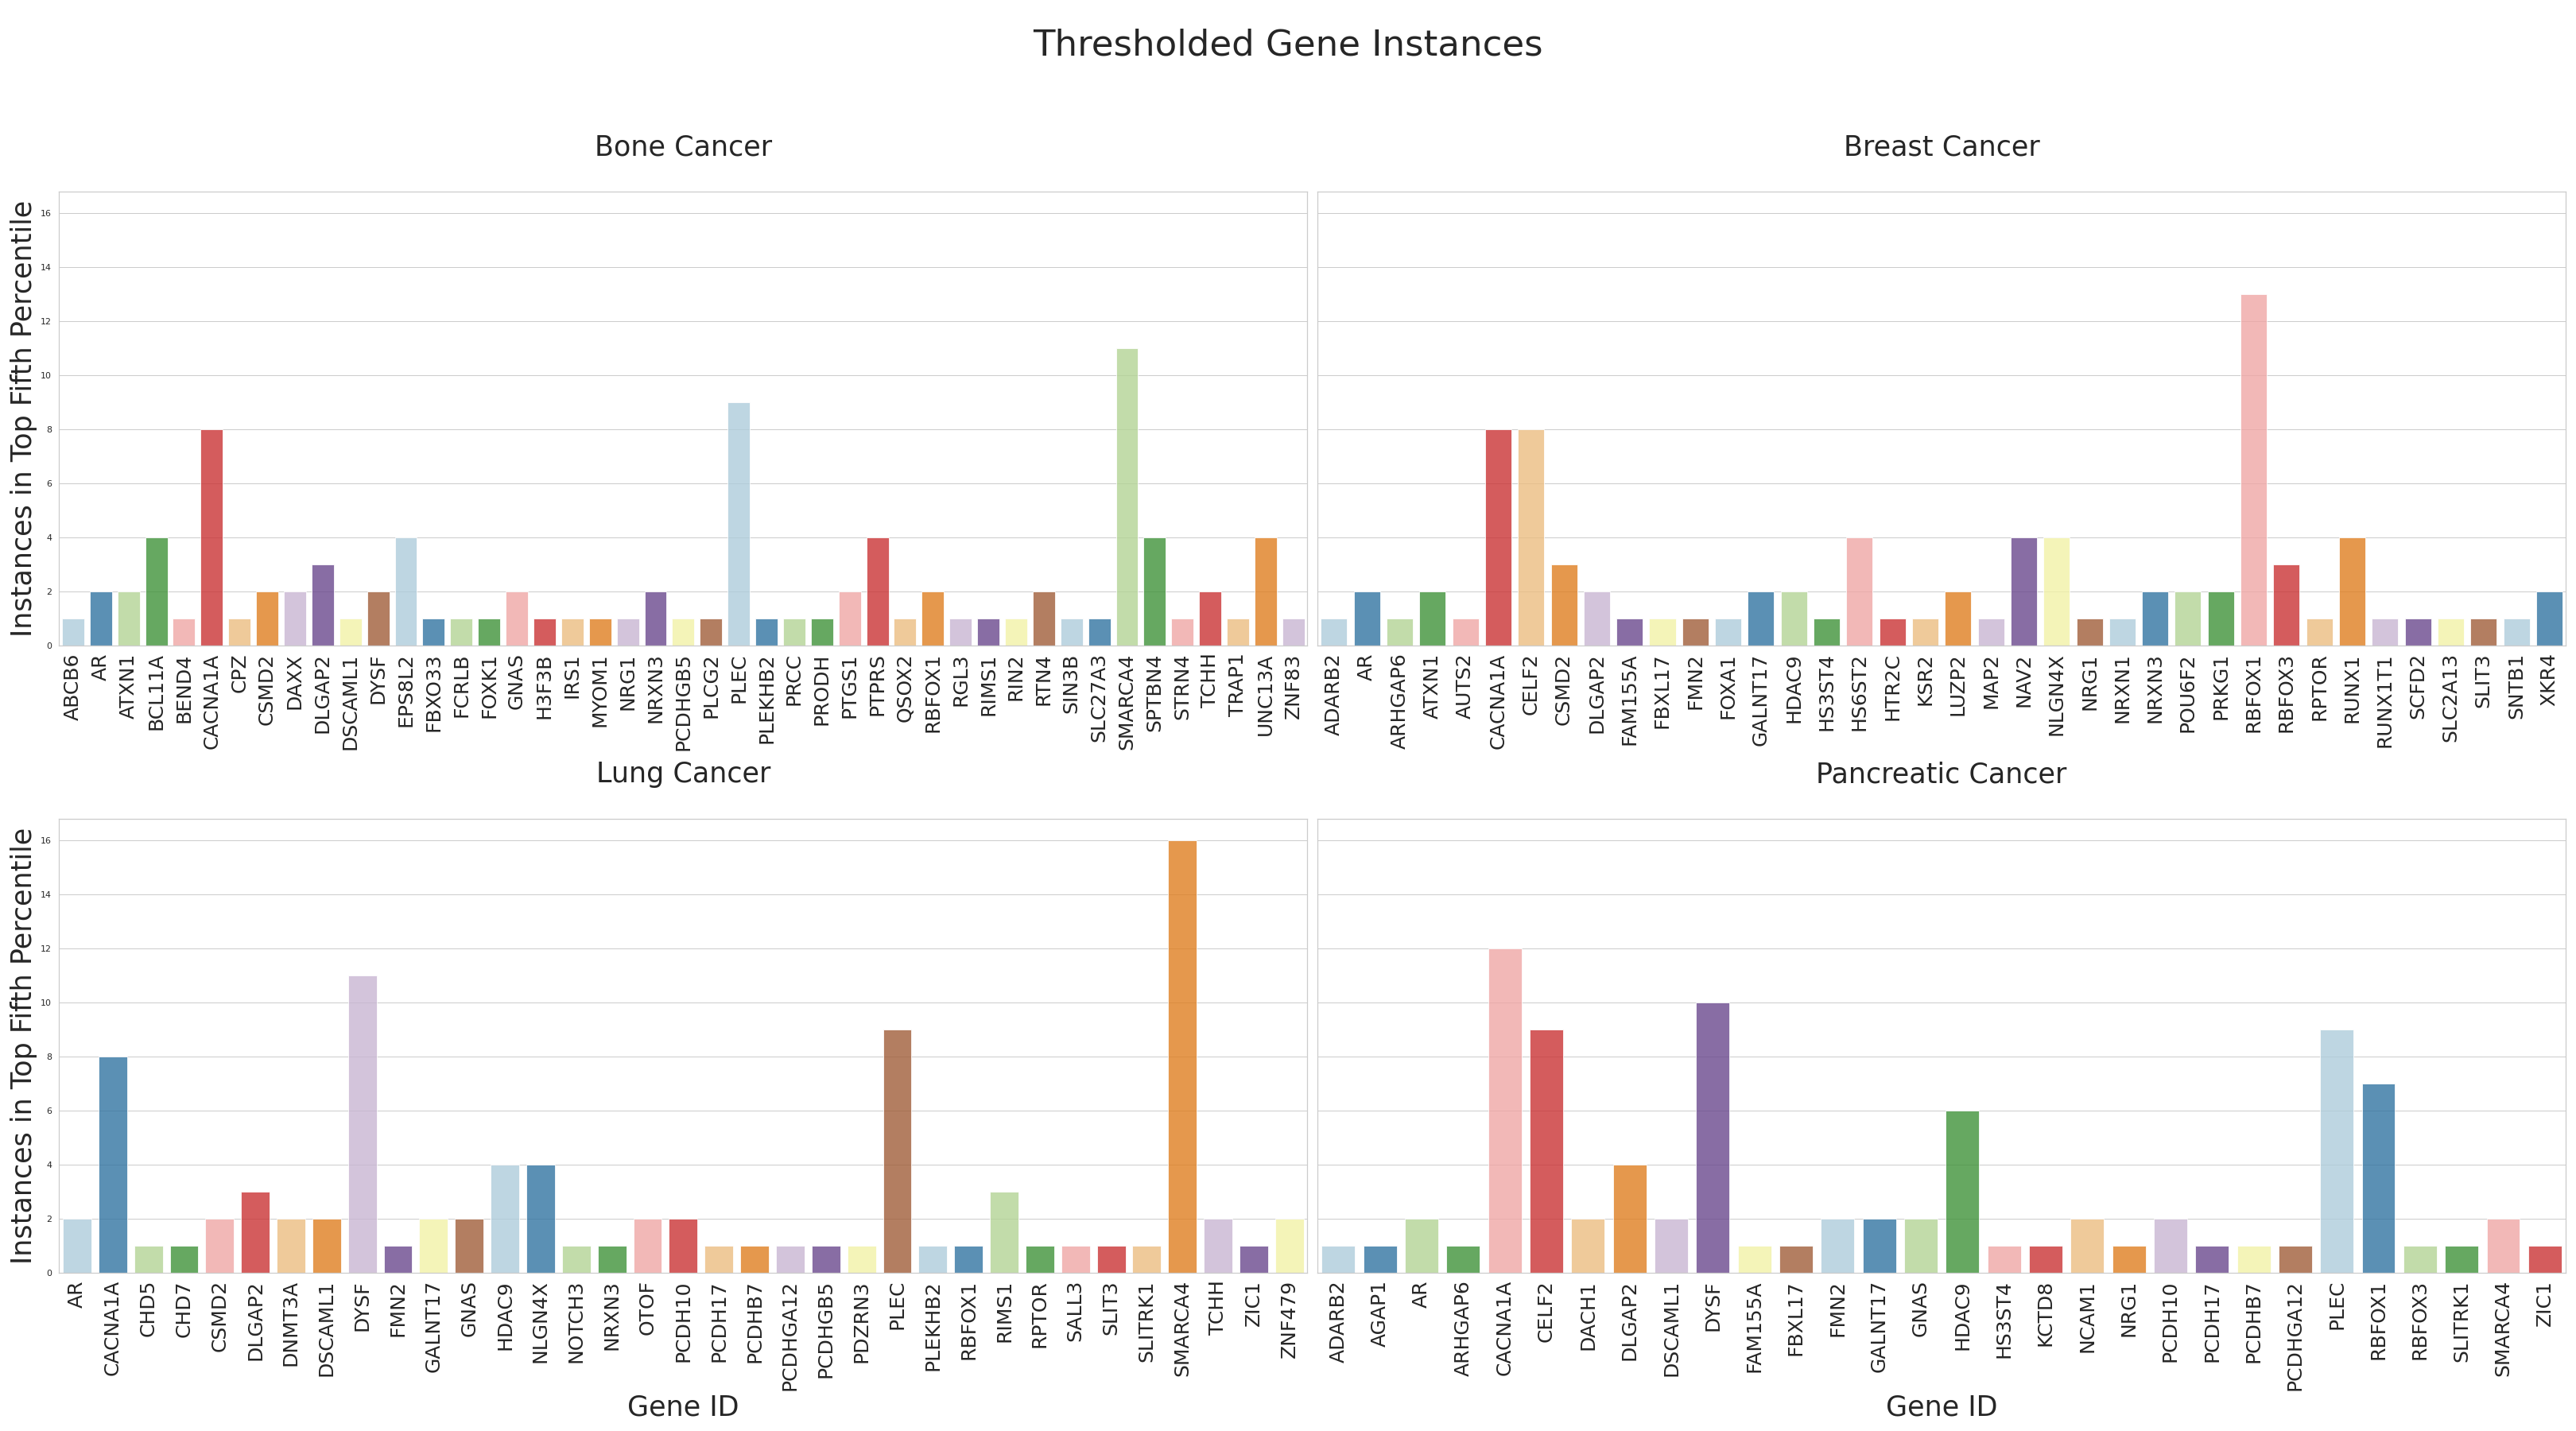
\includegraphics[width=1.2\textwidth]{figures/plots-tight.png}}%
  \caption{Gene frequencies at or above the 95th percentile for sum of feature probability.}
  \label{fig:key}
\end{figure}

In this way, DeepSEA becomes a filter through which a host of genes is newly categorized based on effect size through epigenetic markers. In the CSV which we use to query the Fasta containing all COSMIC cell lines, genes are prioritized based on the proportion of segments that have mutations and the number of overall samples. Here, each of these gene-specific cell lines, represented by the x-axis of Breast Cancer Gene Sums,  is scored not based on the proportion of mutated cell lines, but based on the aggregate probability of epigenetic modification through DeepSEA. 

Having identified this metric as salient, we set out to take the 95 percentile and above of cell lines in each of the aggregate feature matrices for lung cancer, breast cancer, bone cancer, and pancreatic cancer from the COSMIC Genome Browser. After processing this sequence information and outputting tables containing the counts of specific genes among the thresholded cell lines, we produced the plots above, illustrating the instances of a gene in the 95th percentile and above for total feature probability, viewable at a larger size in the appendix. 



\clearpage
\section{References}

\begin{thebibliography}{10}
\bibitem{1}
Leslie, Richard, Christopher J. O’Donnell, and Andrew D. Johnson. "GRASP: analysis of genotype–phenotype results from 1390 genome-wide association studies and corresponding open access database." Bioinformatics 30.12 (2014): i185-i194.
\bibitem{2}
Visscher, Peter M., et al. "Five years of GWAS discovery." The American Journal of Human Genetics 90.1 (2012): 7-24.
\bibitem{3}
Haines, Jonathan L., et al. "Complement factor H variant increases the risk of age-related macular degeneration." Science 308.5720 (2005): 419-421.
\bibitem{4}
Pawelec, Graham. "Immunity and ageing in man." Experimental gerontology 41.12 (2006): 1239-1242.
\bibitem{5}
Klein, Robert J., et al. "Complement factor H polymorphism in age-related macular degeneration." Science 308.5720 (2005): 385-389.
\bibitem{6}
McClellan, Jon, and Mary-Claire King. "Genetic heterogeneity in human disease." Cell 141.2 (2010): 210-217.
\bibitem{7}
Crow, T. J. "The missing genes: what happened to the heritability of psychiatric disorders?." Molecular psychiatry 16.4 (2011): 362-364.
\bibitem{8}
Manolio, Teri A., et al. "Finding the missing heritability of complex diseases." Nature 461.7265 (2009): 747-753.
\bibitem{9}
Alipanahi, Babak, et al. "Predicting the sequence specificities of DNA-and RNA-binding proteins by deep learning." Nature biotechnology 33.8 (2015): 831-838.
\bibitem{10}
Zhou, Jian, and Olga G. Troyanskaya. "Predicting effects of noncoding variants with deep learning–based sequence model." Nature methods 12.10 (2015): 931-934.
\end{thebibliography}

\clearpage
\newpage 
\section{Supplementary Materials}
\textit{Repository: } \href{https://github.com/sme777/CWAS}{\texttt{github.com/sme777/CWAS}}
\\\\\\\\\\\\\\
\begin{figure}[h!]
    \centering
    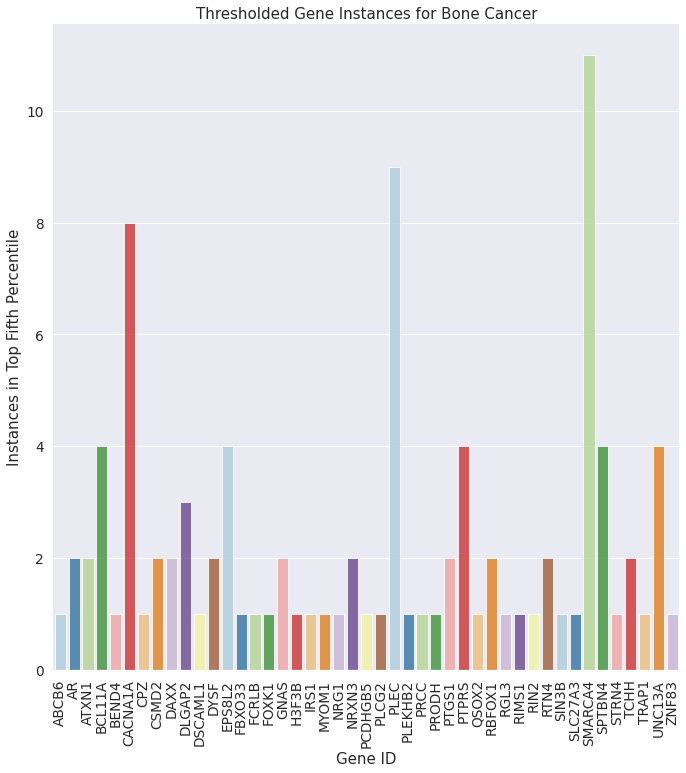
\includegraphics[scale=0.5]{figures/bone.png}
    \caption{Gene frequencies at or above the 95th percentile  for sum of feature probability, bone cancer}
    \label{fig:my_label}
\end{figure}

\begin{figure}[h!]
    \centering
    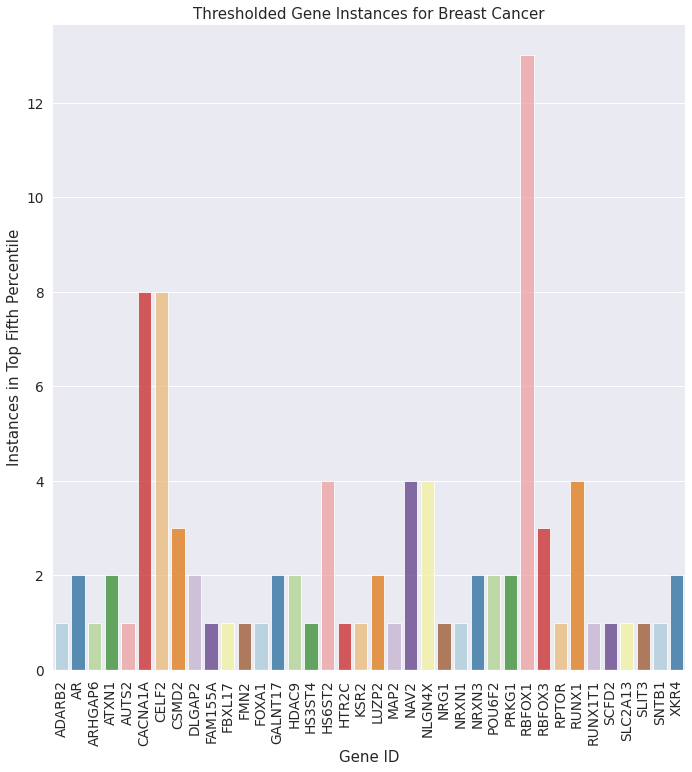
\includegraphics[scale=0.5]{figures/breast.png}
    \caption{Gene frequencies at or above the 95th percentile  for sum of feature probability, breast cancer}
    \label{fig:my_label}
\end{figure}

\begin{figure}[h!]
    \centering
    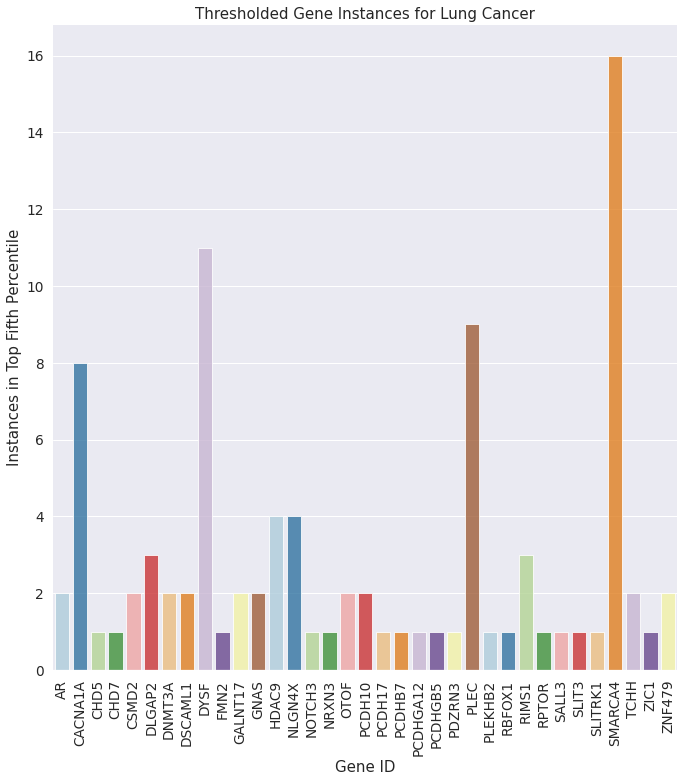
\includegraphics[scale=0.5]{figures/lung.png}
    \caption{Gene frequencies at or above the 95th percentile  for sum of feature probability, lung cancer}
    \label{fig:my_label}
\end{figure}

\begin{figure}[h!]
    \centering
    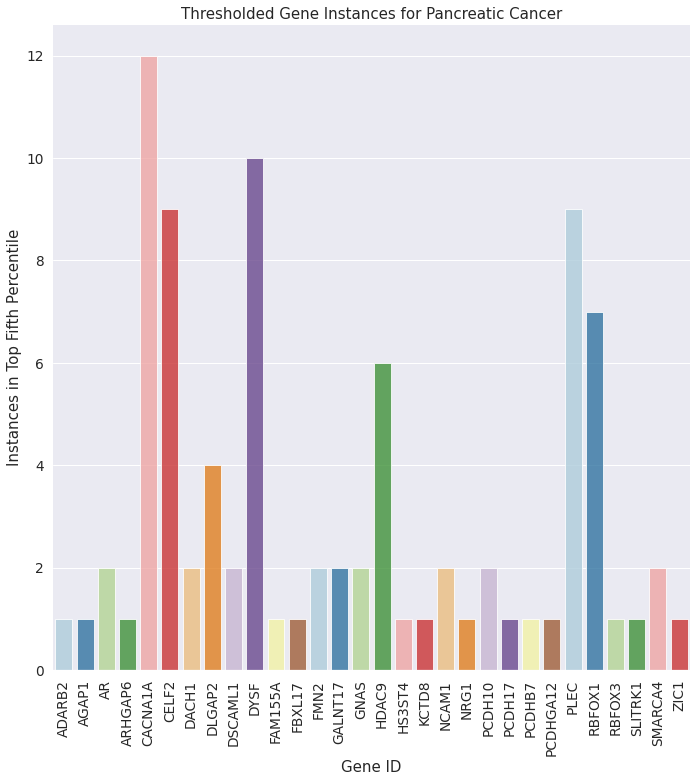
\includegraphics[scale=0.5]{figures/pancreatic.png}
    \caption{Gene frequencies at or above the 95th percentile  for sum of feature probability, pancreatic cancer}
    \label{fig:my_label}
\end{figure}
\end{document}
